\begin{simulation}
\label{sim::ntred} 
\end{simulation}
Considere um manipulador planar com 3 juntas de revolu��o (Figura \ref{fig:sim1_robo}) cuja postura � descrita pela posi��o ${\bf p}\!\in\!\mathbb{R}^2$ e pela orienta��o $\phi\!\in\!\mathbb{R}$.

\begin{figure}[htpb]
  \centering
  \def\Cd{$
 	{\bf x} = 
 	\begin{bmatrix}
 	p_x \\
 	p_y \\
 	\phi \\
 	\end{bmatrix}
 	=
 	\begin{bmatrix}
 	\ell_1\,c1 + \ell_2\,c12 + \ell_3\,c123\\
 	\ell_1\,s1 + \ell_2\,s12 + \ell_3\,s123\\
 	q_1 + q_2 + q_3\\ 
 	\end{bmatrix}
 	= {\bf h}({\bf q})
  $}
  \def\JPicScale{0.69}
  {\small
  \input{fig/simu1_robo.pst}
  }
  \caption{Rob� planar n�o-redundante com 3 juntas de revolu��o}
  \label{fig::manip}
\end{figure}

No que se segue, s�o apresentados resultados de simula��o para rastreamento de posi��o (trajet�ria \ref{traj:1}) e regula��o da orienta��o ($\phi_d = \frac{\pi}{2}$). Considera-se uma configura��o inicial ${\bf q}(0)\,=\,[\frac{\pi}{6}\;\frac{\pi}{6}\;\frac{\pi}{6}]^T rad$.	

\begin{figure}[!htp]
  \centering
  \label{fig::simu1_data}
  \begin{tabular}{cc}
	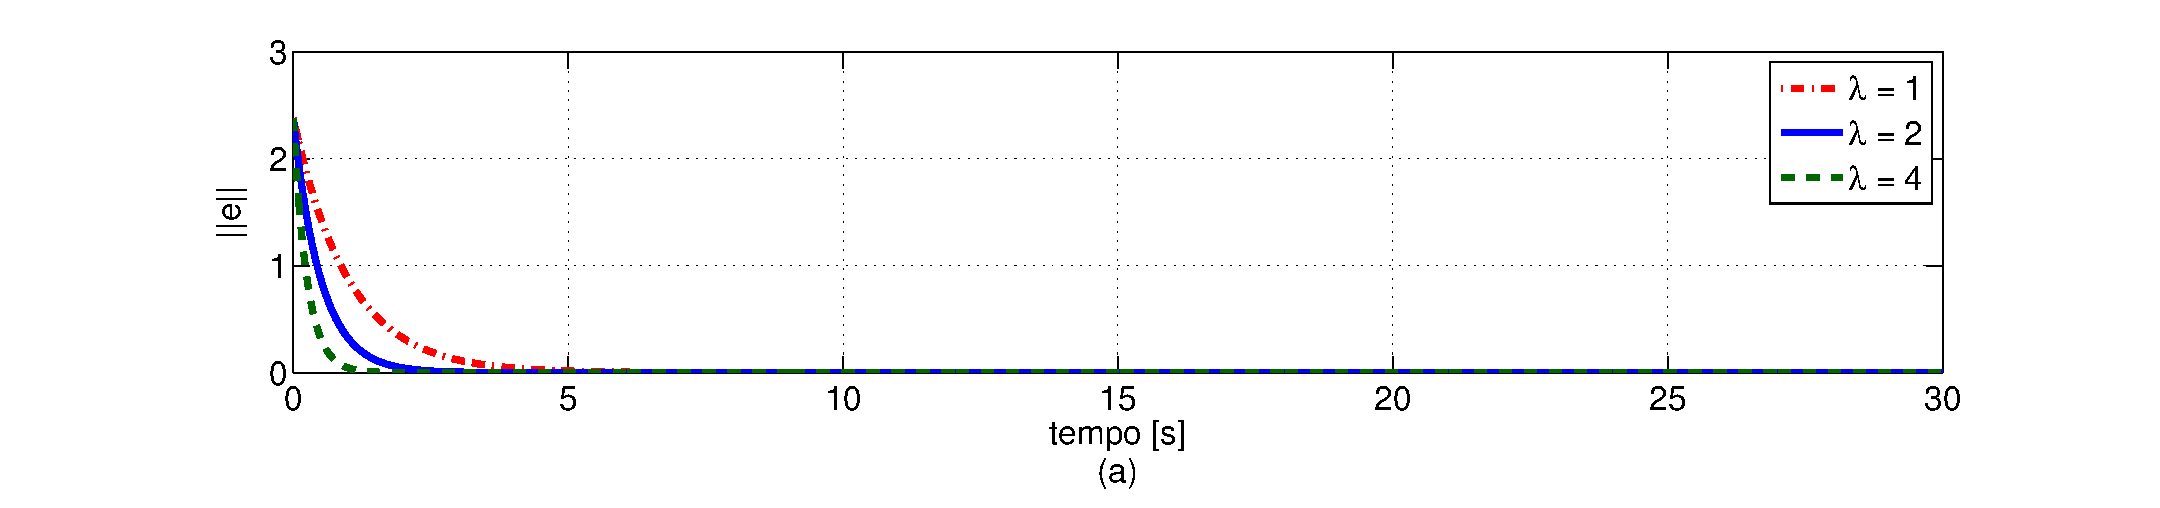
\includegraphics[trim = 2.7cm 0cm 2.7cm 0cm, scale = 0.49]{sim/sim1_norm.eps}\\ %\tiny{\;(a)} \\
	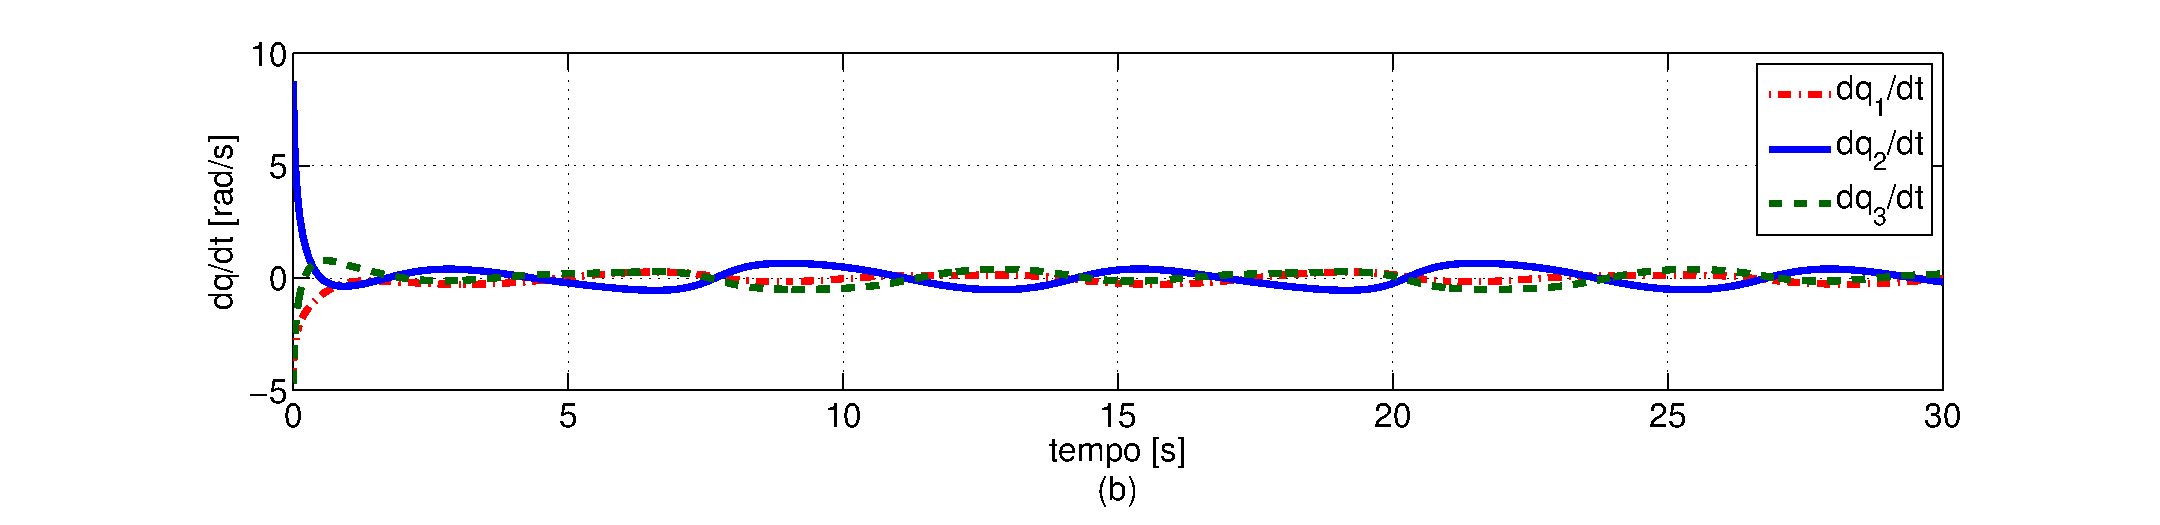
\includegraphics[trim = 2.7cm 0cm 2.7cm 0cm, scale = 0.49]{sim/sim1_qdot.eps}\\ %\tiny{\,(b)} \\
	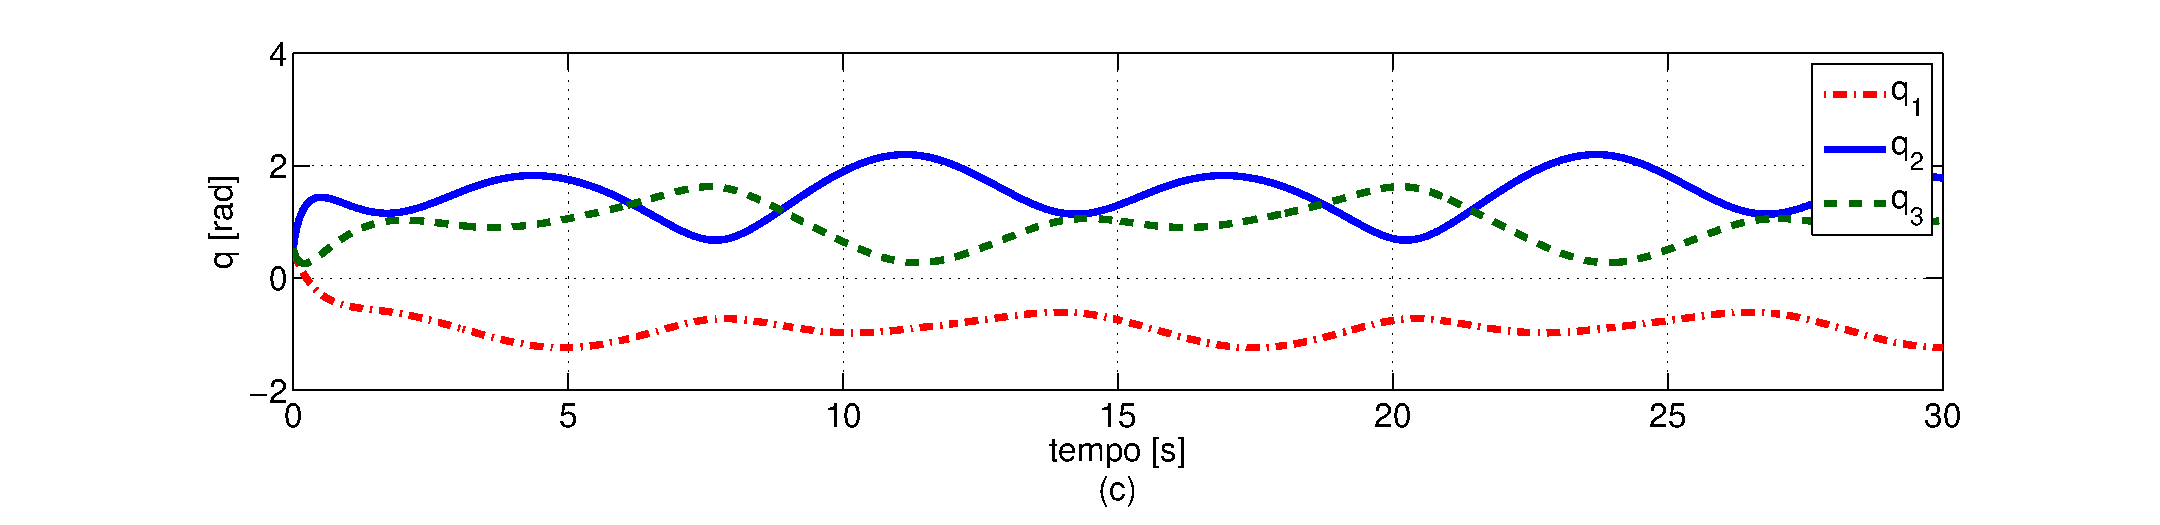
\includegraphics[trim = 2.7cm 0cm 2.7cm 0cm, scale = 0.49]{sim/sim1_q.eps}\\ %\tiny{\!(c)} \\
  \end{tabular}
\caption{Simula��o \ref{sim::ntred}: (a) norma do erro para diferentes ganhos $\lambda$; (b) velocidades das juntas para $\lambda = 2$; e (c) �ngulos das juntas para $\lambda = 2$.}
\end{figure}







\begin{simulation}
\label{sim::red} 
\end{simulation}
Considere um manipulador planar com 3 juntas de revolu��o (Figura \ref{fig::red}) cuja postura � descrita apenas pela posi��o ${\bf p}\!\in\!\mathbb{R}^2$, configurando um problema redundante.

\begin{figure}[htpb]
  \centering
  \def\Cd{$
 	{\bf x} = 
 	\begin{bmatrix}
 	p_x \\
 	p_y \\
 	%\phi \\
 	\end{bmatrix}
 	=
 	\begin{bmatrix}
 	\ell_1\,c1 + \ell_2\,c12 + \ell_3\,c123\\
 	\ell_1\,s1 + \ell_2\,s12 + \ell_3\,s123\\
 	%q_1 + q_2 + q_3\\ 
 	\end{bmatrix}
 	= {\bf h}({\bf q})
  $}
  \def\JPicScale{0.69}
  {\small
  \input{fig/simu1_robo.pst}
  }
  \caption{Rob� planar redundante com 3 juntas de revolu��o}
  \label{fig::red}
\end{figure}

A seguir, s�o apresentados os resultados de simula��o obtidos para rastreamento de posi��o (trajet�ria \ref{traj:1}) e pela lei de norma m�nima (\ref{}). Considera-se novamente uma configura��o inicial ${\bf q}(0)\,=\,[\frac{\pi}{6}\;\frac{\pi}{6}\;\frac{\pi}{6}]^T rad$.	

\begin{figure}[!htp]
  \centering
  \label{fig::simu2_data}
  \begin{tabular}{cc}
	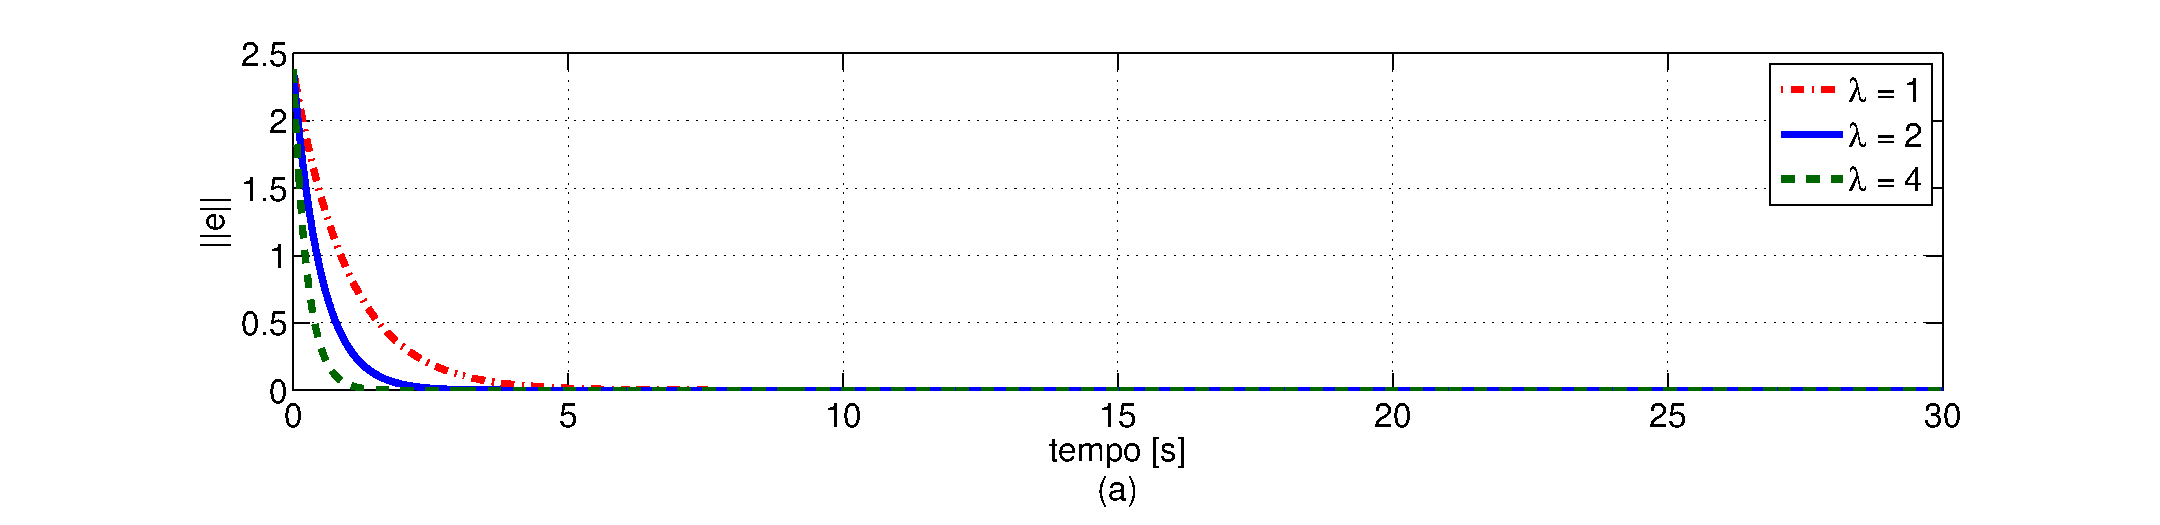
\includegraphics[trim = 2.7cm 0cm 2.7cm 0cm, scale = 0.49]{sim/sim2_norm.eps}\\ %\tiny{\;(a)} \\
	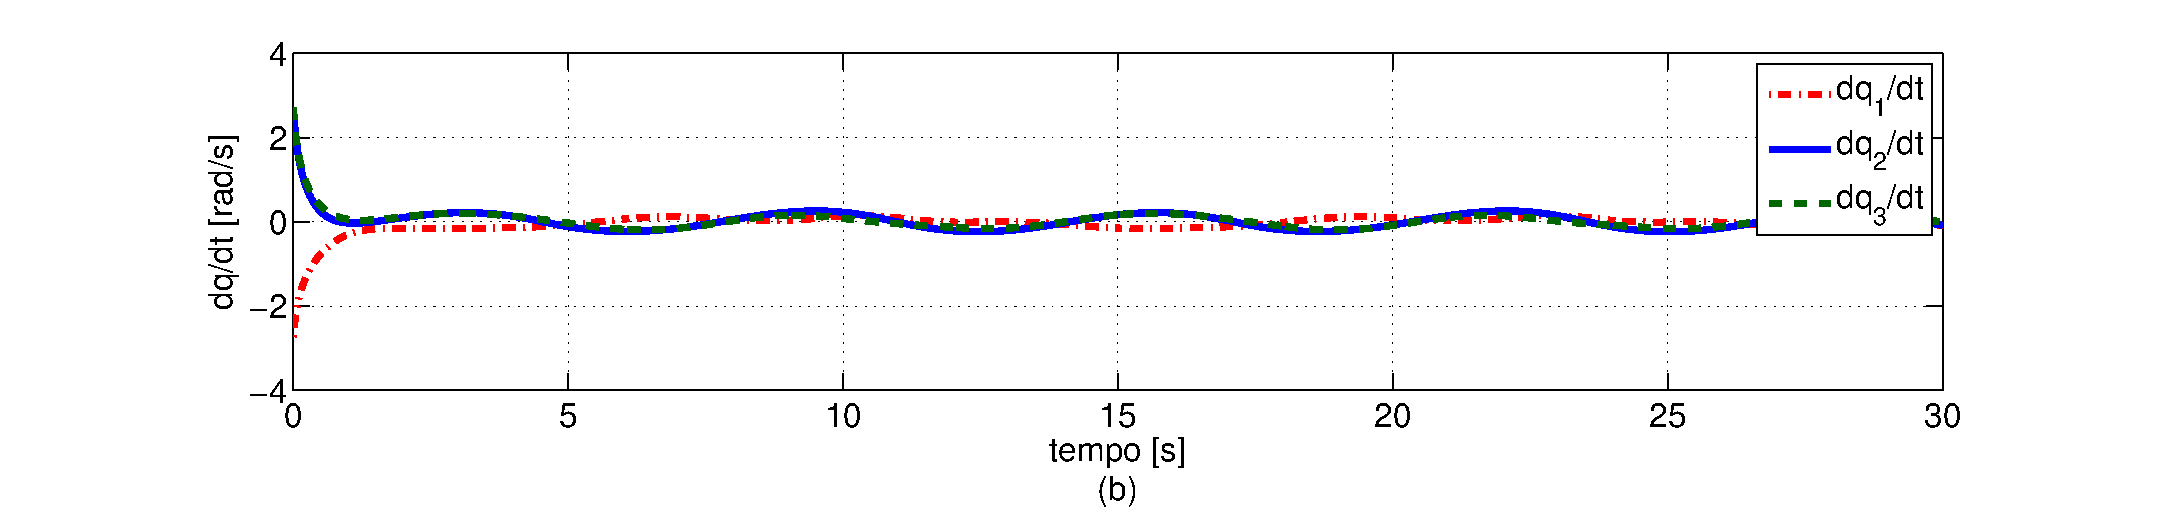
\includegraphics[trim = 2.7cm 0cm 2.7cm 0cm, scale = 0.49]{sim/sim2_qdot.eps}\\ %\tiny{\,(b)} \\
	\includegraphics[trim = 2.7cm 0cm 2.7cm 0cm, scale = 0.49]{sim/sim2_q.eps}\\ %\tiny{\!(c)} \\
  \end{tabular}
\caption{Simula��o \ref{sim::ntred}: (a) norma do erro para diferentes ganhos $\lambda$; (b) velocidades das juntas para $\lambda = 2$; e (c) �ngulos das juntas para $\lambda = 2$.}
\end{figure}







